\addcontentsline{toc}{section}{Appendix}

\chead{\textit{\nouppercase{Appendix}}}

\thispagestyle{plain} % surpress header on first page

\subsection{Appendix A: Tables} \label{appendixA}
\thispagestyle{plain} % surpress header on first page

\begin{table}[H]
	\centering
	\caption{Correlation between Parameter Estimates}
	\label{table2}
	\begin{tabular}{l | c c c c c c c}
		\toprule\midrule
		& $\hat{RC}$ & $\hat\theta_{11}$ & $\hat\theta_{30}$ & $\hat\theta_{31}$ & $\hat\theta_{32}$ & $\hat\theta_{33}$ \\ \midrule
		$\hat{RC}$ & 1.0 & 0.97 & -0.04 & -0.01 & 0.00 & 0.15 \\
		$\hat\theta_{11}$ & 0.97 & 1.0 & -0.02 & -0.03 & 0.01 &	0.14 \\
		$\hat\theta_{30}$ &	-0.04 &	-0.02 &	1.0	& -0.26 & -0.31 & -0.07 \\
		$\hat\theta_{31}$ &	-0.01 &	-0.03 &	-0.26 &	1.0 & -0.82 & -0.06 \\
		$\hat\theta_{32}$ &	0.00 & 0.01 & -0.31 & -0.82 & 1.0 &	-0.12 \\
		$\hat\theta_{33}$ &	0.15 & 0.14 & -0.07 & -0.06 & -0.12 & 1.0 \\
		\bottomrule
	\end{tabular}
\end{table}


\begin{table}[H]
	\centering
	\caption{The Specifications for the Sensitivity Simulation}
	\label{table3}
	\begin{tabular}{l c c c c}
		\toprule\midrule
		Specification & $\beta$ & Cost Function & Grid Size & Analytical \\
		& & & & Gradient \\ \midrule
		0 & 0.975 & linear& 100& Yes\\
		1&0.975& linear& 100& No\\
		2&0.975& linear& 200& Yes\\
		3&0.975& linear& 200& No\\
		4&0.975& linear& 400& Yes\\
		5&0.975& linear& 400& No\\
		6&0.975& quadratic& 100& Yes\\
		7&0.975& quadratic& 100& No\\
		8&0.975& quadratic& 200& Yes\\
		9&0.975& quadratic& 200& No\\
		10&0.975& quadratic& 400& Yes\\
		11&0.975& quadratic& 400& No\\
		12&0.975& cubic& 100& Yes\\
		13&0.975& cubic& 100& No\\
		14&0.975& cubic& 200& Yes\\
		15&0.975& cubic& 200& No\\
		16&0.975& cubic& 400& Yes\\
		17&0.975& cubic& 400& No\\
		18&0.985& linear& 100& Yes\\
		19&0.985& linear& 100& No\\
		20&0.985& linear& 200& Yes\\
		21&0.985& linear& 200& No\\
		22&0.985& linear& 400& Yes\\
		23&0.985& linear& 400& No\\
		24&0.985& quadratic& 100& Yes\\
		25&0.985& quadratic& 100& No\\
		26&0.985& quadratic& 200& Yes\\
		27&0.985& quadratic& 200& No\\
		28&0.985& quadratic& 400& Yes\\
		29&0.985& quadratic& 400& No\\
		30&0.985& cubic& 100& Yes\\
		31&0.985& cubic& 100& No\\
		32&0.985& cubic& 200& Yes\\
		33&0.985& cubic& 200& No\\
		34&0.985& cubic& 400& Yes\\
		35&0.985& cubic& 400& No\\
		\bottomrule
	\end{tabular}
\end{table}


\begin{table}[H]
	\centering
	\caption{Mean Quantitative Comparison for Specifications of Figure 8}
	\label{table4}
	\begin{tabular}{l | c c c c c c}
		\toprule\midrule
		Specification & Time & Major & Func. & Func. & Bellm. & N.K.   \\
		& (in Sec.) & Iter. & Eval. & Eval. (total) & Iter. & Iter. \\
		\midrule
		4 \& NFXP & 7.38 & 11.73 &	13.25 &	NaN & 285.04 & 76.98 \\
		4 \& MPEC & 23.13 & 18.68 & 23.75 & 23.75 & NaN & NaN \\
		5 \& NFXP & 16.43 &  11.73 & 13.25 & NaN & 1080.16 & 286.84 \\
		5 \& MPEC & 168.39 & 19.13 &	24.63 &	8540.83 & NaN &	NaN \\
		3 \& NFXP & 3.72 & 14.02 & 15.02 & NaN &	1221.28 & 322.91 \\
		3 \& MPEC & 26.37 & 22.1 & 28.01 & 4919.5 & NaN & NaN \\
		1 \& NFXP & 1.19 & 12.35 & 13.82 & NaN &	1125.92 & 282.24 \\
		1 \& MPEC & 4.44 & 21.56 & 31.5 & 2457.77 & NaN & NaN \\
		\bottomrule
	\end{tabular}
\end{table}

\newpage
\subsection{Appendix B: Figures}

\begin{figure}[H]
	\caption{The QoI when varying the Cost Function (BHHH)}
	\vspace*{-4mm}
	\centering
	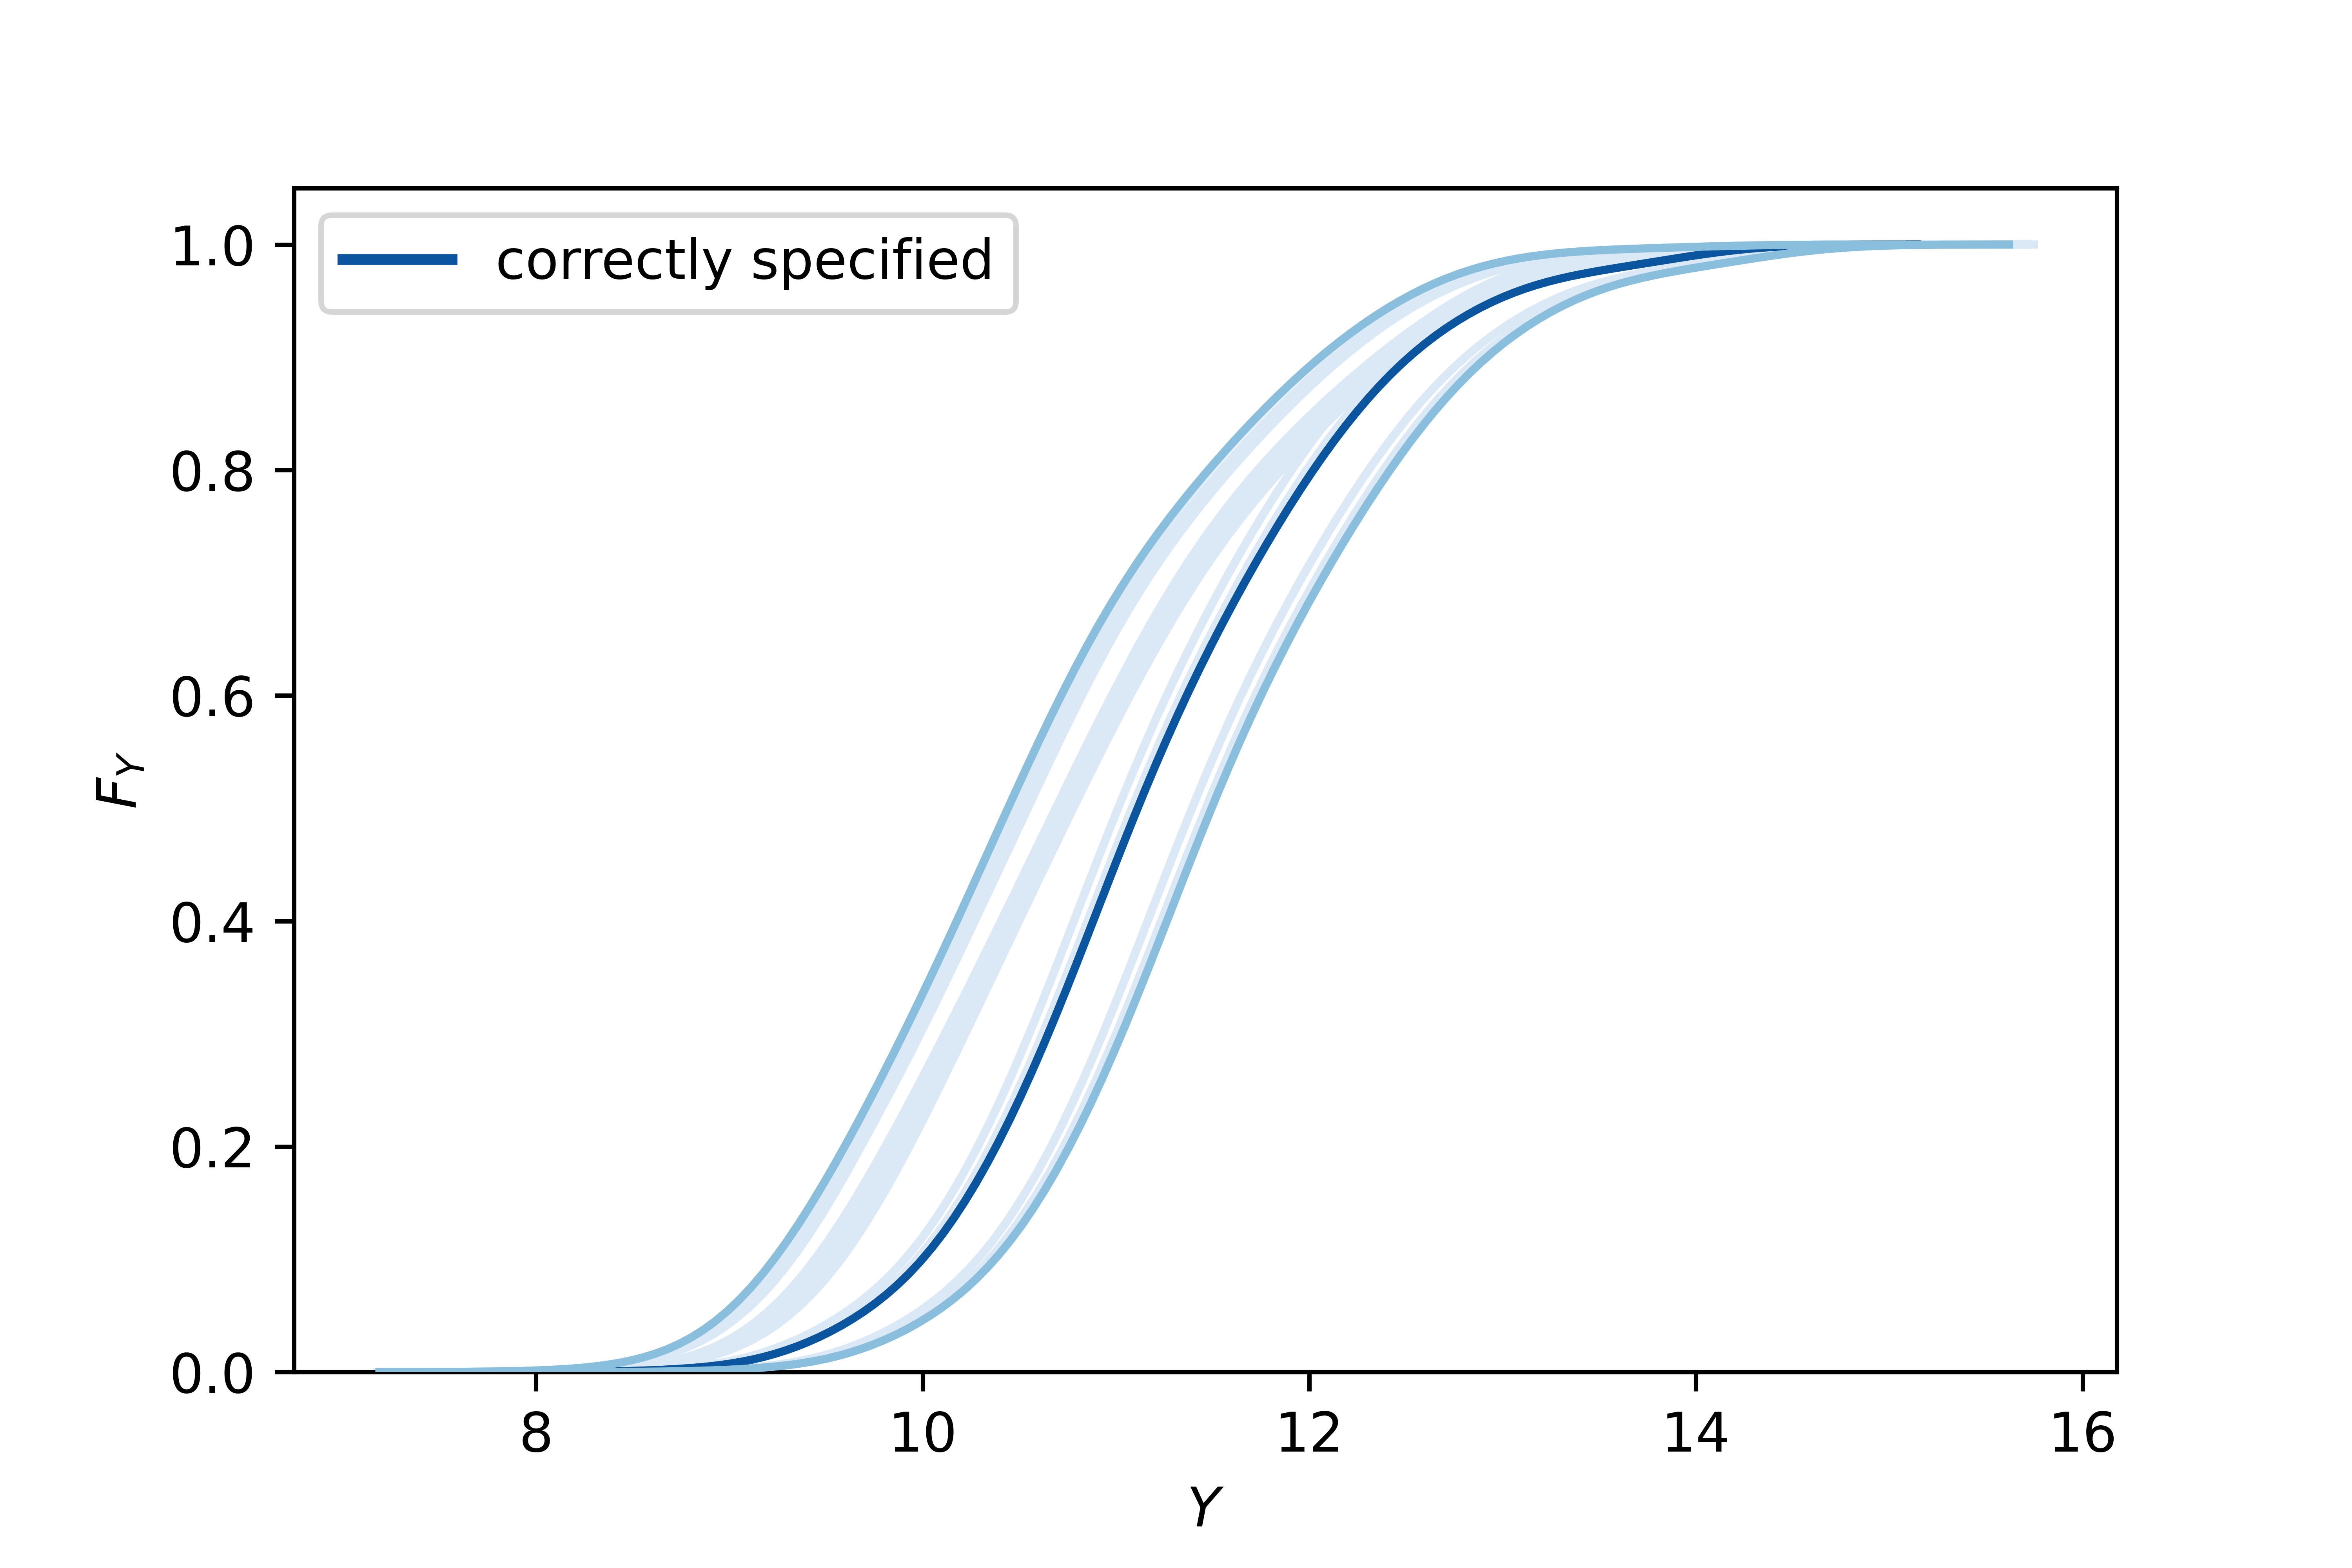
\includegraphics[scale=0.9]{../figures/figure_12.png}
	\label{figure12}
\end{figure}

\begin{figure}[H]
	\caption{The PDF and CDF of the QoI with the NFXP}
	\vspace*{-4mm}
	\centering
	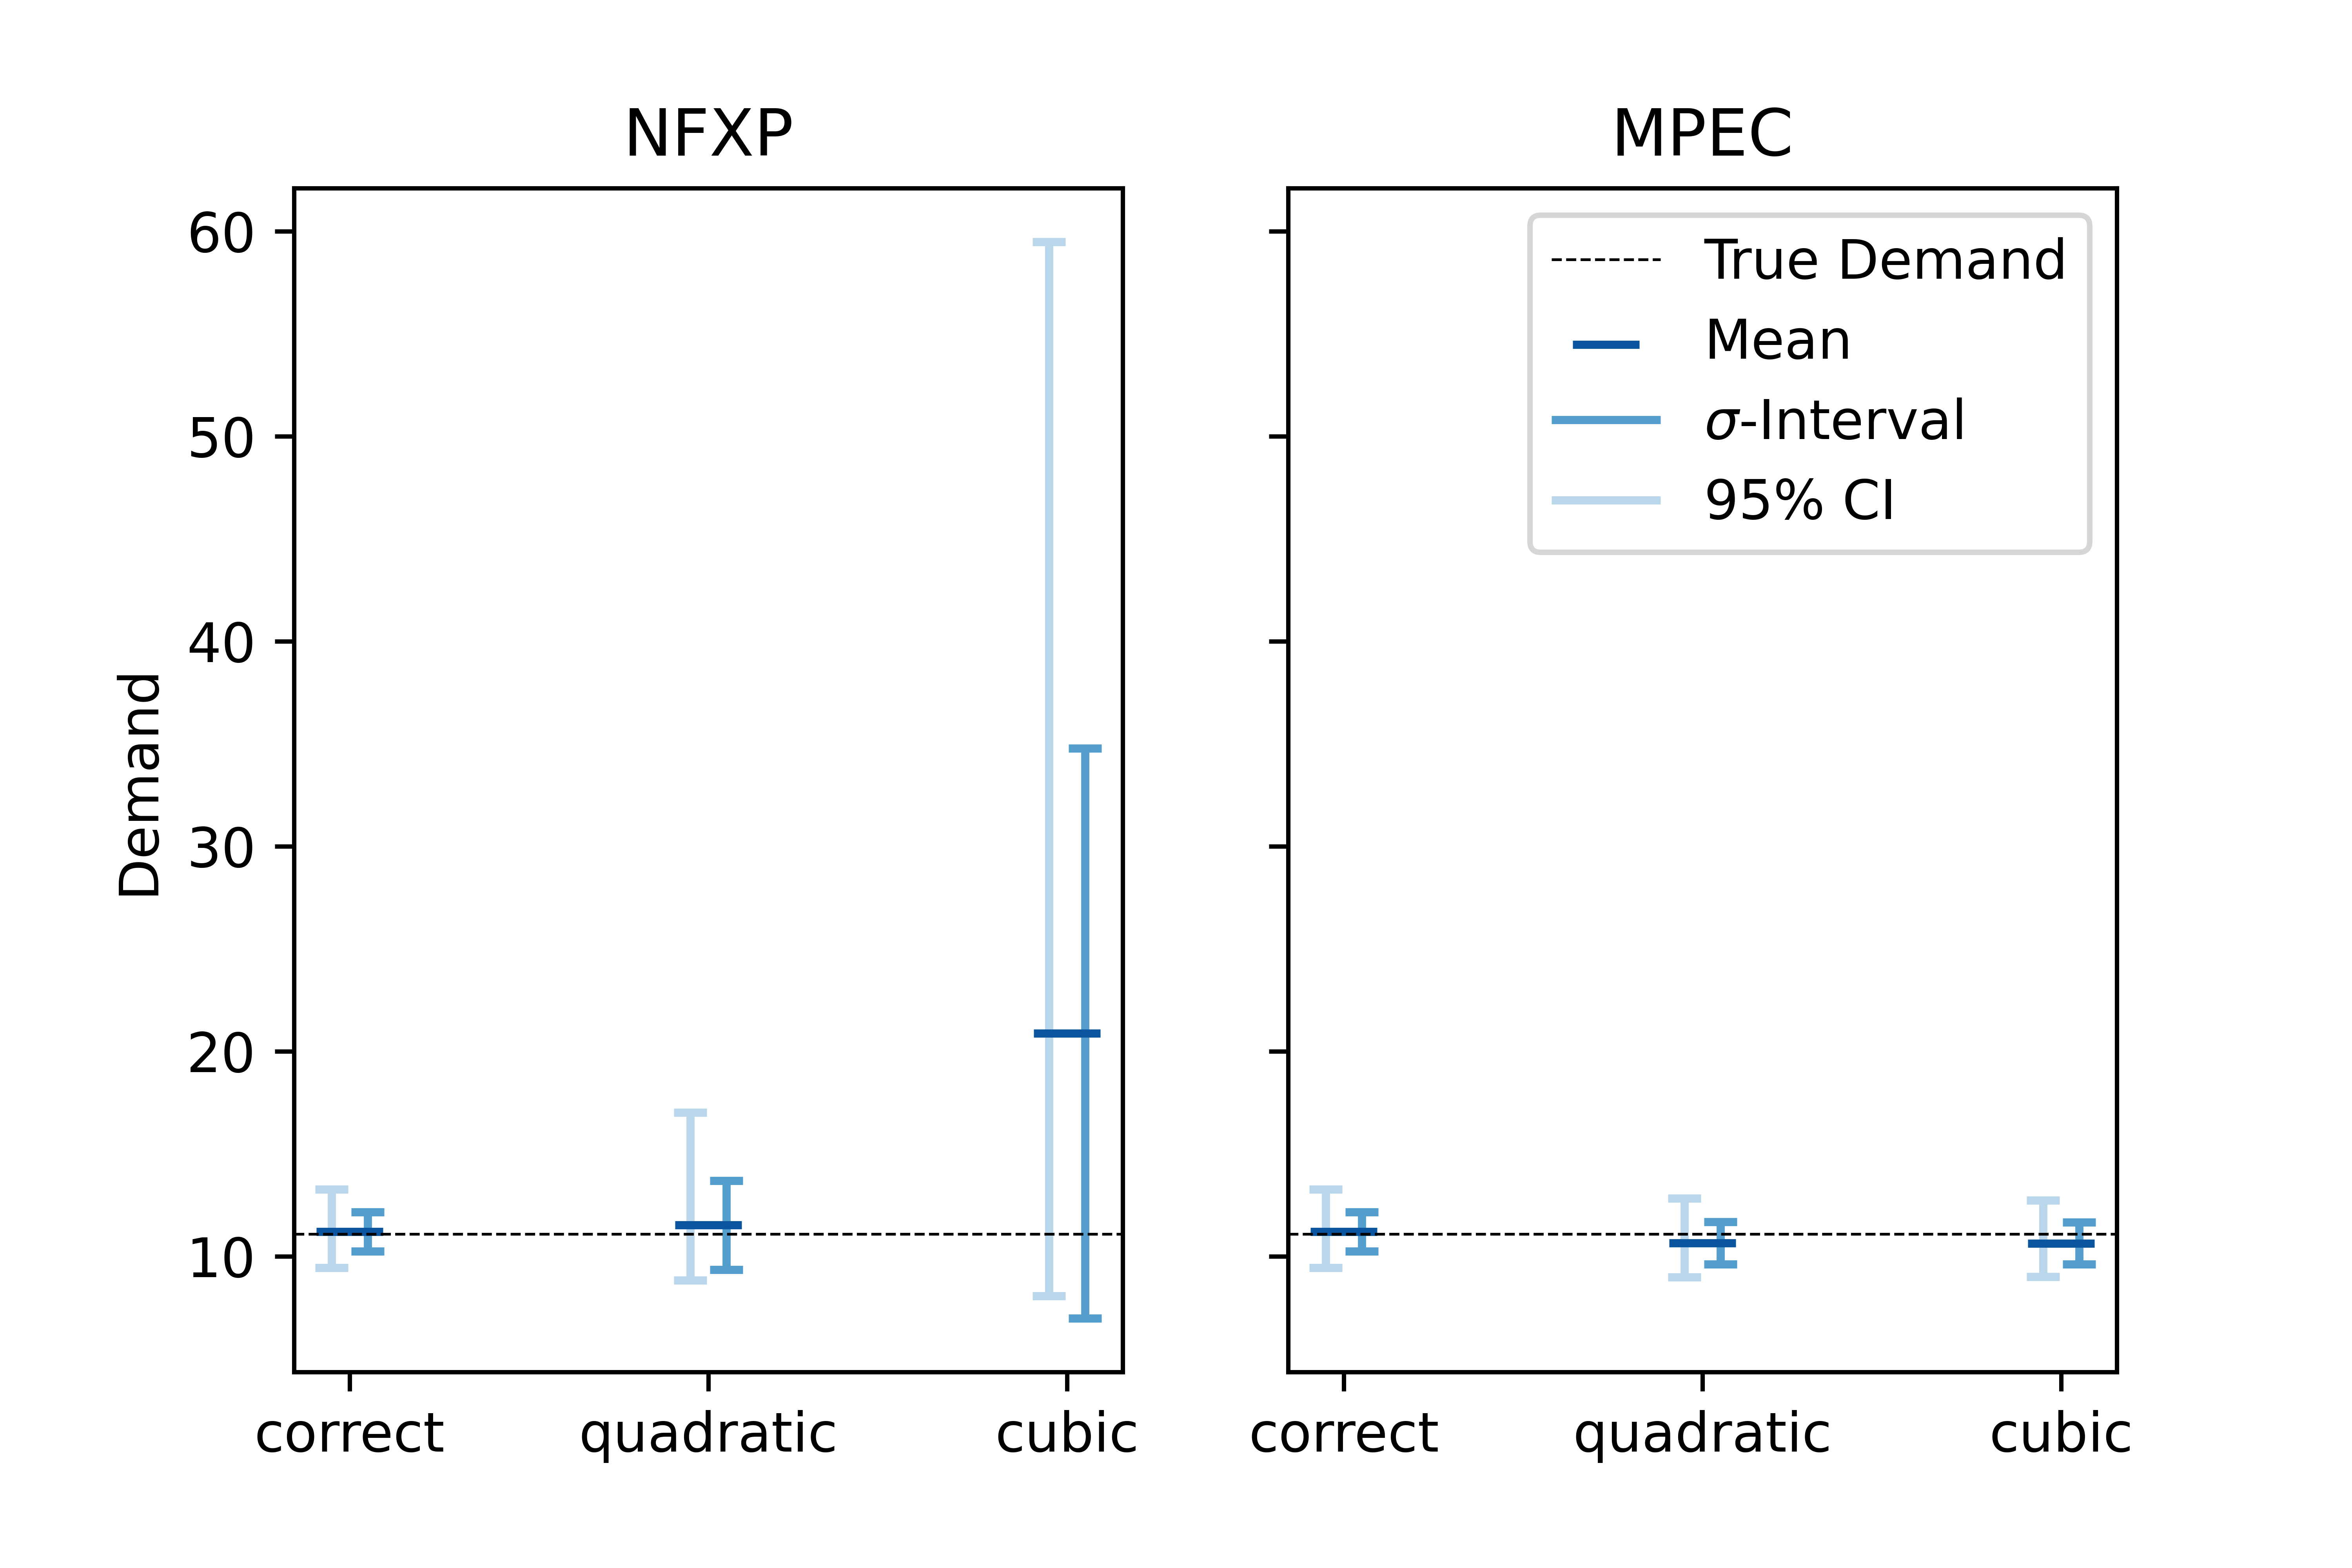
\includegraphics[scale=0.9]{../figures/figure_13.png}
	\label{figure13}
\end{figure}


\newpage
\subsection{Appendix C: Further Details on the Replication of Iskhakov et al. (2016)} \label{appendixC}

This part explains to which extent my implementations of the NFXP and MPEC differ to the ones by \cite{Iskhakov.2016}. As already laid out in section \ref{generalsetup}, I rely entirely on open-source programs which has some implications for my methodology. The authors use matlab for the NFXP (they also implement the BHHH like this) and the modeling language AMPL in combination with the solver KNITRO for MPEC. I, on the other hand, implement everything in Python only and use IPOPT as a solver for MPEC. This alone can cause their results and mine to differ. Additionally, for MPEC they obtain first and second order analytical derivatives of the Lagrangian as AMPL provides them using automatic differentiation. While there are tools such as JAX\footnote{ See \url{https://github.com/google/jax}.} that provide analytical derivatives via automatic differentiation for code written in Python, these restrict the code to have a certain form which would have involved rewriting main parts of the existing code. This might be an interesting extension of the package for later but is out of scope for this thesis. I decided therefore to at least code up the first order derivative by hand and pass it in to IPOPT. The fact that in my case the Hessian has to be approximated can potentially influence the results strongly. \citeauthor{Iskhakov.2016} also give sparsity patterns of the two derivatives to KNITRO in order to conserve memory and increase speed. This is not done in my implementation. Another practical difference comes from the fact that KNITRO and IPOPT rely on different stopping criteria which makes it impossible to exactly replicate the setup for KNITRO with IPOPT. For the NFXP there are also some differences. My BHHH as well as the switching from contraction to N-K iterations has other tolerances. On top of that, \citeauthor{Iskhakov.2016} allow the fixed point algorithm to switch back from N-K to contraction steps when a certain criteria is met. This flexibility is not implemented in my code.

In the light of that, the algorithms by \citeauthor{Iskhakov.2016} are slightly more complex and robust which might affect the number of iterations and function evaluations for MPEC and especially the amount of contraction and N-K steps needed in the case of the NFXP. This can be observed in Table \ref{table1}. Although one should mention that the more comparable implementation of MPEC in which \cite{Su.Judd.2012} use matlab as the modeling language and KNITRO with only first order analytical derivatives as solver seems to be inferior to my implementation when looking at the number of iterations and function evaluations needed.\footnote{ To see this, have a look at Table II on page 2228 of \cite{Su.Judd.2012} One has to be cautious, though, as their implementation differs from mine in the sense that they do not recenter the expected value function. Although this should generally only cause the solver to converge more often due to increased numerically stability but should not affect the parameter estimates and should not change the speed too much.} For an additional sanity check I provide the mean and standard deviations of the estimated cost parameters across the Monte Carlo simulations outlined in section \ref{generalsetup}. These are meaningful as \cite{Su.Judd.2012} argue that this simulation actually constitutes a parametric bootstrap procedure.

\begin{table}[!t]
	\label{table5}
	\centering
	\caption{Comparison to the Results of Iskhakov et al. (2016)}
	\begin{tabular}{l c c c c}
		\toprule\midrule
		& & & RC & $\theta_{11}$ \\
		\cmidrule{4-5}
		$\beta$ & Implementation & True Values: & $\mathbf{11.726}$ & $\mathbf{2.457}$ \\ \midrule
		0.975 & MPEC & Mean & 11.908 & 2.507 \\
		& & Std. Dev. & (1.517) & (0.486) \\
		& NFXP & Mean & 11.908 & 2.507 \\
		& & Std. Dev. & (1.517) & (0.468) \\
		& NFXP Iskhakov & Mean & 11.914 & 2.508 \\
		& & Std. Dev. & (1.517) & (0.468) \\ \midrule
		0.985 & MPEC & Mean & 11.986 & 2.534 \\
		& & Std. Dev. & (1.457) & (0.452) \\
		& NFXP & Mean & 11.986 & 2.534 \\
		& & Std. Dev. & (1.457) & (0.452) \\
		& NFXP Iskhakov & Mean & 11.991 & 2.535 \\
		& & Std. Dev. & (1.457) & (0.452) \\ \midrule
		0.995 & MPEC & Mean & 11.891 & 2.508 \\
		& & Std. Dev. & (1.384) & (0.440) \\
		& NFXP & Mean & 11.891 & 2.508 \\
		& & Std. Dev. & (1.384) & (0.440) \\
		& NFXP Iskhakov & Mean & 11.191	& 2.902 \\
		& & Std. Dev. & (1.188) & (0.473) \\ \midrule
		0.999 & MPEC & Mean & 11.874 & 2.513 \\
		& & Std. Dev. & (1.347) & (0.444) \\
		& NFXP & Mean & 11.874 & 2.513 \\
		& & Std. Dev. & (1.347) & (0.444) \\
		& NFXP Iskhakov & Mean & 11.876	& 2.513 \\
		& & Std. Dev. & (1.346) & (0.444) \\ \midrule
		0.9995 & MPEC & Mean & 11.849 & 2.509 \\
		& & Std. Dev. & (1.343) & (0.445) \\
		& NFXP & Mean & 11.847 & 2.508 \\
		& & Std. Dev. & (1.343) & (0.445) \\
		& NFXP Iskhakov & Mean & 11.849 & 2.509 \\
		& & Std. Dev. & (1.342) & (0.445) \\ \midrule
		0.9999 & MPEC & Mean & 11.815 & 2.498 \\
		& & Std. Dev. & (1.319) & (0.431) \\
		& NFXP & Mean & 11.815 & 2.499 \\
		& & Std. Dev. & (1.319) & (0.431) \\
		& NFXP Iskhakov & Mean & 11.817	& 2.499 \\
		& & Std. Dev. & (1.319) & (0.431) \\ \bottomrule
	\end{tabular}
\end{table}

The two statistics are provided for both my implementations and additionally for the NFXP of \cite{Iskhakov.2016}. Those results were not published but had to be obtained by me using their matlab replication code. Unfortunately, their code does not run through but only did with some additional changes. This should make one a bit cautious regarding those results. All of those results are presented in the table below in which can be seen that apart from when $\beta$ equals $0.995$, the results of all three approaches are very similar.

My implementations overestimate the true parameter slightly for $RC$ while coming gradually closer to the true value with increasing $\beta$. This pattern can also be seen in Table I of \cite{Su.Judd.2012} (who base their analysis on the same data generating process) which makes me confident that my results are correct. It seems like for $\beta = 0.995$ the NFXP Iskhakov is trapped in another local minimum that causes it to overestimate the true $\theta_{11}$ by a lot and suddenly underestimate the true $RC$. As mentioned before, this is likely to be caused by the fact that their code did not run through and it is not obviously clear whether the setup in the code is exactly like the one the published results are based on.

\subsection{Appendix D: MPEC for respy} \label{appendixD}

In a preliminary stage of my thesis, I explored whether it could be beneficial to use MPEC instead of the NFXP for a python package called respy (see \cite{Gabler.2020}) developed at the University of Bonn. This package offers users to flexibly estimate models from the class of Eckstein-Keane-Wolpin (EKW) models as defined in \cite{Aguirregabiri.2010}. While I initially set up a notebook with a simulation based on the one of \cite{Iskhakov.2016} in order to explore the applicability and usefulness of MPEC for respy\footnote{ See \url{https://github.com/Pascalheid/MPEC_for_respy/blob/master/mpec_fo_respy.ipynb}.}, similar arguments can be made with my major simulation in this thesis.

While the EKW models also belong to the class of single agent dynamic discrete choice models, they differ to the Rust model by relaxing some of its key assumptions. To give a few examples, first of all, they allow agents to have several choices that are mutually exclusive. Further, \cite{Aguirregabiri.2010} highlight that, as for instance in \cite{Keane.1994}, there is permanent unobserved heterogeneity of individuals and unobservables can be correlated across choice alternatives. The assumption that the unobservables are not necessarily extreme value distributed further relaxes Rust's assumptions. This provokes the first complexity in solving the model to obtain conditional choice probabilities with which the likelihood function can be obtained. The economic model must be solved for multiple types (due to heterogeneity) each time and solving the model involves numerically solving multi-dimension integrals (as no closed form solution exists due to the flexibility in distribution of the unobservables). This is needed to obtain an integrated value function coined \textit{EMAX} by \cite{Keane.1994} for the calculation of the conditional choice probabilities. As the model has a finite horizon, it also does not involve a fixed point calculation but rather can be solved using backward induction for the integrated value functions. While it should generally be possible to cast the backward induction with its integrated value function calculation into the constraint of an augmented likelihood function, it is reasonable to first explore whether an MPEC formulation of this problem in general might prove beneficial in this setting. Establishing the problem as a MPEC would involve having a new parameter per integrated value function. This results in an immense amount of parameters and constraints. To see this, let us have a look at the context of the EKW models. Those are set in Labor Economics and at each point in time an agent has the option to work in a specific profession or stay at home. Those are the several possible discrete choices. The state space consists at each point in time of a history of experience in a certain job or schooling and the choice given that history. In order to solve the problem by backward induction, only obtaining the last periods choice specific value functions, it is necessary to calculate the integrated value function at each possible state space (job and schooling history)  that might occur in the last period (compare \cite{Aguirregabiri.2010, Keane.1994, Keane.1997}). Depending on the amount of alternative choices and time periods, the state space is extremely large. In any case, it will be way beyond the $175$ constraints and $177$ parameters modeled in \cite{Su.Judd.2012} and \cite{Iskhakov.2016}.

Another factor is that the criterion function that has to be optimized in the respy package is not differentiable everywhere which likely stays like that when switching to MPEC. This gives rise to another complication that the above mentioned authors did not have to face. I have to rely on finite-difference numerical derivatives while the authors in the Rust setting could even rely on the desirable feature of analytical first and second order derivatives. Additionally, the sparsity patterns of those are supplied to the solver. All this together makes their setting quite favorable in the sense that the implementation is as efficient as it could be yielding the very high speed and convergence. While \cite{Su.Judd.2012} report to have successfully run MPEC in this setting of the Rust model with 100,052 parameters and 100,042 constraints within an hour on 12 GB RAM work station (which is the range of dimensions, one would face in reasonable implementations of EKW models), this will likely not be possible in the less favorable setting of respy.

There are several possible reasons to arrive at this opinion. Those are already laid out to a certain extent in section \ref{partial} (it makes sense to read that section before the following) and can be observed in Table \ref{table4}. The increased dimensionality of the MPEC formulation in comparison to the NFXP in combination with finite-difference numerical derivatives results in a surge of function evaluations. While those function evaluations are far less costly than those of the NFXP in the Rust model, this is less clearly so in respy. In the Rust model the trade-off stems from the speed and robustness with which the fixed point calculation is implemented. As the model in respy is solved via backward induction, the efficiency gain that might arise from casting it into the constraints as opposed to coding it up yourself is less clear. \cite{Su.Judd.2012} report that the main advantage of MPEC is that it does not enforce the fixed point to hold exactly until the last iteration of the calibration process. \cite{Aguirregabiria.2002} argue that this is computationally more efficient as it is not necessary to enforce it precisely in each iteration. From this it is also not directly clear whether this also holds true for backward induction of Bellman equations, weakening another key argument for MPEC. Another observation that can be made in Table \ref{table4} is that the fact of using numerical derivatives paired with increasing number of constraints and parameters (here represented by increasing grid size) seems to affect the performance of MPEC more heavily than it does the one of NFXP. The critical factor here is the previously mentioned trade-off between the massive amount of function evaluations for MPEC and the increased complexity of solving the fixed point for the NFXP. Seeing that already in this setting with only a low dimensionality (in comparison to the one expected in respy) the CPU time and major iterations for MPEC climb up more strongly than for NFXP, does not seem to make it beneficial to further seriously test the usefulness of MPEC for respy. Although initially considered to implement MPEC in repsy as a topic for my thesis, it was not deemed to be valuable to pursue for the above outlined reasons.

